\documentclass[twoside]{book}

% Packages required by doxygen
\usepackage{calc}
\usepackage{doxygen}
\usepackage{graphicx}
\usepackage[utf8]{inputenc}
\usepackage{makeidx}
\usepackage{multicol}
\usepackage{multirow}
\usepackage{textcomp}
\usepackage[table]{xcolor}

% Font selection
\usepackage[T1]{fontenc}
\usepackage{mathptmx}
\usepackage[scaled=.90]{helvet}
\usepackage{courier}
\usepackage{amssymb}
\usepackage{sectsty}
\renewcommand{\familydefault}{\sfdefault}
\allsectionsfont{%
  \fontseries{bc}\selectfont%
  \color{darkgray}%
}
\renewcommand{\DoxyLabelFont}{%
  \fontseries{bc}\selectfont%
  \color{darkgray}%
}

% Page & text layout
\usepackage{geometry}
\geometry{%
  a4paper,%
  top=2.5cm,%
  bottom=2.5cm,%
  left=2.5cm,%
  right=2.5cm%
}
\tolerance=750
\hfuzz=15pt
\hbadness=750
\setlength{\emergencystretch}{15pt}
\setlength{\parindent}{0cm}
\setlength{\parskip}{0.2cm}
\makeatletter
\renewcommand{\paragraph}{%
  \@startsection{paragraph}{4}{0ex}{-1.0ex}{1.0ex}{%
    \normalfont\normalsize\bfseries\SS@parafont%
  }%
}
\renewcommand{\subparagraph}{%
  \@startsection{subparagraph}{5}{0ex}{-1.0ex}{1.0ex}{%
    \normalfont\normalsize\bfseries\SS@subparafont%
  }%
}
\makeatother

% Headers & footers
\usepackage{fancyhdr}
\pagestyle{fancyplain}
\fancyhead[LE]{\fancyplain{}{\bfseries\thepage}}
\fancyhead[CE]{\fancyplain{}{}}
\fancyhead[RE]{\fancyplain{}{\bfseries\leftmark}}
\fancyhead[LO]{\fancyplain{}{\bfseries\rightmark}}
\fancyhead[CO]{\fancyplain{}{}}
\fancyhead[RO]{\fancyplain{}{\bfseries\thepage}}
\fancyfoot[LE]{\fancyplain{}{}}
\fancyfoot[CE]{\fancyplain{}{}}
\fancyfoot[RE]{\fancyplain{}{\bfseries\scriptsize Generated on Thu Jul 11 2013 12:11:32 for Sudoku by Doxygen }}
\fancyfoot[LO]{\fancyplain{}{\bfseries\scriptsize Generated on Thu Jul 11 2013 12:11:32 for Sudoku by Doxygen }}
\fancyfoot[CO]{\fancyplain{}{}}
\fancyfoot[RO]{\fancyplain{}{}}
\renewcommand{\footrulewidth}{0.4pt}
\renewcommand{\chaptermark}[1]{%
  \markboth{#1}{}%
}
\renewcommand{\sectionmark}[1]{%
  \markright{\thesection\ #1}%
}

% Indices & bibliography
\usepackage{natbib}
\usepackage[titles]{tocloft}
\setcounter{tocdepth}{3}
\setcounter{secnumdepth}{5}
\makeindex

% Hyperlinks (required, but should be loaded last)
\usepackage{ifpdf}
\ifpdf
  \usepackage[pdftex,pagebackref=true]{hyperref}
\else
  \usepackage[ps2pdf,pagebackref=true]{hyperref}
\fi
\hypersetup{%
  colorlinks=true,%
  linkcolor=blue,%
  citecolor=blue,%
  unicode%
}

% Custom commands
\newcommand{\clearemptydoublepage}{%
  \newpage{\pagestyle{empty}\cleardoublepage}%
}


%===== C O N T E N T S =====

\begin{document}

% Titlepage & ToC
\hypersetup{pageanchor=false}
\pagenumbering{roman}
\begin{titlepage}
\vspace*{7cm}
\begin{center}%
{\Large Sudoku \\[1ex]\large 0.\-3 }\\
\vspace*{1cm}
{\large Generated by Doxygen 1.8.4}\\
\vspace*{0.5cm}
{\small Thu Jul 11 2013 12:11:32}\\
\end{center}
\end{titlepage}
\clearemptydoublepage
\tableofcontents
\clearemptydoublepage
\pagenumbering{arabic}
\hypersetup{pageanchor=true}

%--- Begin generated contents ---
\chapter{Hierarchical Index}
\section{Class Hierarchy}
This inheritance list is sorted roughly, but not completely, alphabetically\-:\begin{DoxyCompactList}
\item \contentsline{section}{Cell}{\pageref{class_cell}}{}
\item Q\-Dialog\begin{DoxyCompactList}
\item \contentsline{section}{Inicio}{\pageref{class_inicio}}{}
\end{DoxyCompactList}
\item Q\-Main\-Window\begin{DoxyCompactList}
\item \contentsline{section}{Main\-Window}{\pageref{class_main_window}}{}
\end{DoxyCompactList}
\item \contentsline{section}{qt\-\_\-meta\-\_\-stringdata\-\_\-\-Inicio\-\_\-t}{\pageref{structqt__meta__stringdata___inicio__t}}{}
\item \contentsline{section}{qt\-\_\-meta\-\_\-stringdata\-\_\-\-Main\-Window\-\_\-t}{\pageref{structqt__meta__stringdata___main_window__t}}{}
\item \contentsline{section}{Sudoku}{\pageref{class_sudoku}}{}
\item \contentsline{section}{Sudoku\-Generator}{\pageref{class_sudoku_generator}}{}
\item \contentsline{section}{Ui\-\_\-\-Inicio}{\pageref{class_ui___inicio}}{}
\begin{DoxyCompactList}
\item \contentsline{section}{Ui\-:\-:Inicio}{\pageref{class_ui_1_1_inicio}}{}
\end{DoxyCompactList}
\item \contentsline{section}{Ui\-\_\-\-Main\-Window}{\pageref{class_ui___main_window}}{}
\begin{DoxyCompactList}
\item \contentsline{section}{Ui\-:\-:Main\-Window}{\pageref{class_ui_1_1_main_window}}{}
\end{DoxyCompactList}
\end{DoxyCompactList}

\chapter{Class Index}
\section{Class List}
Here are the classes, structs, unions and interfaces with brief descriptions\-:\begin{DoxyCompactList}
\item\contentsline{section}{\hyperlink{class_cell}{Cell} }{\pageref{class_cell}}{}
\item\contentsline{section}{\hyperlink{class_inicio}{Inicio} }{\pageref{class_inicio}}{}
\item\contentsline{section}{\hyperlink{class_ui_1_1_inicio}{Ui\-::\-Inicio} }{\pageref{class_ui_1_1_inicio}}{}
\item\contentsline{section}{\hyperlink{class_main_window}{Main\-Window} }{\pageref{class_main_window}}{}
\item\contentsline{section}{\hyperlink{class_ui_1_1_main_window}{Ui\-::\-Main\-Window} }{\pageref{class_ui_1_1_main_window}}{}
\item\contentsline{section}{\hyperlink{structqt__meta__stringdata___inicio__t}{qt\-\_\-meta\-\_\-stringdata\-\_\-\-Inicio\-\_\-t} }{\pageref{structqt__meta__stringdata___inicio__t}}{}
\item\contentsline{section}{\hyperlink{structqt__meta__stringdata___main_window__t}{qt\-\_\-meta\-\_\-stringdata\-\_\-\-Main\-Window\-\_\-t} }{\pageref{structqt__meta__stringdata___main_window__t}}{}
\item\contentsline{section}{\hyperlink{class_sudoku}{Sudoku} }{\pageref{class_sudoku}}{}
\item\contentsline{section}{\hyperlink{class_sudoku_generator}{Sudoku\-Generator} }{\pageref{class_sudoku_generator}}{}
\item\contentsline{section}{\hyperlink{class_ui___inicio}{Ui\-\_\-\-Inicio} }{\pageref{class_ui___inicio}}{}
\item\contentsline{section}{\hyperlink{class_ui___main_window}{Ui\-\_\-\-Main\-Window} }{\pageref{class_ui___main_window}}{}
\end{DoxyCompactList}

\chapter{Class Documentation}
\hypertarget{class_cell}{\section{Cell Class Reference}
\label{class_cell}\index{Cell@{Cell}}
}
\subsection*{Public Member Functions}
\begin{DoxyCompactItemize}
\item 
\hyperlink{class_cell_a394510643e8664cf12b5efaf5cb99f71}{Cell} ()
\begin{DoxyCompactList}\small\item\em Constructor de la clase \hyperlink{class_cell}{Cell} por defecto. \end{DoxyCompactList}\item 
\hyperlink{class_cell_aa4c34c694dde0a9f3729f86775a57aa0}{Cell} (int x, int y, int value)
\begin{DoxyCompactList}\small\item\em Constructor de la clase \hyperlink{class_cell}{Cell} con parámetros. \end{DoxyCompactList}\item 
int \hyperlink{class_cell_a78d82b277e8fb2e1c3e70286bcc85314}{get\-X} () const 
\begin{DoxyCompactList}\small\item\em devuelve el atributo x. \end{DoxyCompactList}\item 
int \hyperlink{class_cell_a2df3d69f5d0c10a1e1f02c5f89045e0a}{get\-Y} () const 
\begin{DoxyCompactList}\small\item\em devuelve el atributo y. \end{DoxyCompactList}\item 
int \hyperlink{class_cell_a1a906844dab60dbd4f3590194d8a81bb}{get\-Value} () const 
\begin{DoxyCompactList}\small\item\em devuelve el atributo value. \end{DoxyCompactList}\item 
void \hyperlink{class_cell_af6cc63822a2cf6a5acef52c030316cbe}{set\-X} (int x)
\begin{DoxyCompactList}\small\item\em Setter del atributo x. \end{DoxyCompactList}\item 
void \hyperlink{class_cell_aee8634042d34858b42eab29f5409de9e}{set\-Y} (int y)
\begin{DoxyCompactList}\small\item\em Setter del atributo y. \end{DoxyCompactList}\item 
void \hyperlink{class_cell_a9b58034e57c99329a534189428882e0e}{set\-Value} (int value)
\begin{DoxyCompactList}\small\item\em Setter del atributo Value. \end{DoxyCompactList}\item 
bool \hyperlink{class_cell_a28ca469fc17820e26d08ebf34adc8807}{equals} (\hyperlink{class_cell}{Cell} d)
\end{DoxyCompactItemize}


\subsection{Constructor \& Destructor Documentation}
\hypertarget{class_cell_a394510643e8664cf12b5efaf5cb99f71}{\index{Cell@{Cell}!Cell@{Cell}}
\index{Cell@{Cell}!Cell@{Cell}}
\subsubsection[{Cell}]{\setlength{\rightskip}{0pt plus 5cm}Cell\-::\-Cell (
\begin{DoxyParamCaption}
{}
\end{DoxyParamCaption}
)}}\label{class_cell_a394510643e8664cf12b5efaf5cb99f71}


Constructor de la clase \hyperlink{class_cell}{Cell} por defecto. 

\begin{DoxyAuthor}{Author}
Iván Aveiga. 
\end{DoxyAuthor}
\hypertarget{class_cell_aa4c34c694dde0a9f3729f86775a57aa0}{\index{Cell@{Cell}!Cell@{Cell}}
\index{Cell@{Cell}!Cell@{Cell}}
\subsubsection[{Cell}]{\setlength{\rightskip}{0pt plus 5cm}Cell\-::\-Cell (
\begin{DoxyParamCaption}
\item[{int}]{x, }
\item[{int}]{y, }
\item[{int}]{value}
\end{DoxyParamCaption}
)}}\label{class_cell_aa4c34c694dde0a9f3729f86775a57aa0}


Constructor de la clase \hyperlink{class_cell}{Cell} con parámetros. 

\begin{DoxyAuthor}{Author}
Iván Aveiga. 
\end{DoxyAuthor}


\subsection{Member Function Documentation}
\hypertarget{class_cell_a28ca469fc17820e26d08ebf34adc8807}{\index{Cell@{Cell}!equals@{equals}}
\index{equals@{equals}!Cell@{Cell}}
\subsubsection[{equals}]{\setlength{\rightskip}{0pt plus 5cm}bool Cell\-::equals (
\begin{DoxyParamCaption}
\item[{{\bf Cell}}]{d}
\end{DoxyParamCaption}
)}}\label{class_cell_a28ca469fc17820e26d08ebf34adc8807}
Retorna si this es igual a c en valor y posición. 
\begin{DoxyParams}{Parameters}
{\em c} & Celda a comparar. \\
\hline
\end{DoxyParams}
\begin{DoxyReturn}{Returns}
booleano si son iguales. 
\end{DoxyReturn}
\begin{DoxyAuthor}{Author}
Iván Aveiga.
\end{DoxyAuthor}
\hypertarget{class_cell_a1a906844dab60dbd4f3590194d8a81bb}{\index{Cell@{Cell}!get\-Value@{get\-Value}}
\index{get\-Value@{get\-Value}!Cell@{Cell}}
\subsubsection[{get\-Value}]{\setlength{\rightskip}{0pt plus 5cm}int Cell\-::get\-Value (
\begin{DoxyParamCaption}
{}
\end{DoxyParamCaption}
) const}}\label{class_cell_a1a906844dab60dbd4f3590194d8a81bb}


devuelve el atributo value. 

\begin{DoxyReturn}{Returns}
atributo value. 
\end{DoxyReturn}
\begin{DoxyAuthor}{Author}
Iván Aveiga. 
\end{DoxyAuthor}
\hypertarget{class_cell_a78d82b277e8fb2e1c3e70286bcc85314}{\index{Cell@{Cell}!get\-X@{get\-X}}
\index{get\-X@{get\-X}!Cell@{Cell}}
\subsubsection[{get\-X}]{\setlength{\rightskip}{0pt plus 5cm}int Cell\-::get\-X (
\begin{DoxyParamCaption}
{}
\end{DoxyParamCaption}
) const}}\label{class_cell_a78d82b277e8fb2e1c3e70286bcc85314}


devuelve el atributo x. 

\begin{DoxyReturn}{Returns}
atributo x. 
\end{DoxyReturn}
\begin{DoxyAuthor}{Author}
Iván Aveiga. 
\end{DoxyAuthor}
\hypertarget{class_cell_a2df3d69f5d0c10a1e1f02c5f89045e0a}{\index{Cell@{Cell}!get\-Y@{get\-Y}}
\index{get\-Y@{get\-Y}!Cell@{Cell}}
\subsubsection[{get\-Y}]{\setlength{\rightskip}{0pt plus 5cm}int Cell\-::get\-Y (
\begin{DoxyParamCaption}
{}
\end{DoxyParamCaption}
) const}}\label{class_cell_a2df3d69f5d0c10a1e1f02c5f89045e0a}


devuelve el atributo y. 

\begin{DoxyReturn}{Returns}
atributo y. 
\end{DoxyReturn}
\begin{DoxyAuthor}{Author}
Iván Aveiga. 
\end{DoxyAuthor}
\hypertarget{class_cell_a9b58034e57c99329a534189428882e0e}{\index{Cell@{Cell}!set\-Value@{set\-Value}}
\index{set\-Value@{set\-Value}!Cell@{Cell}}
\subsubsection[{set\-Value}]{\setlength{\rightskip}{0pt plus 5cm}void Cell\-::set\-Value (
\begin{DoxyParamCaption}
\item[{int}]{value}
\end{DoxyParamCaption}
)}}\label{class_cell_a9b58034e57c99329a534189428882e0e}


Setter del atributo Value. 


\begin{DoxyParams}{Parameters}
{\em value} & valor a setear en el atributo value. \\
\hline
\end{DoxyParams}
\begin{DoxyAuthor}{Author}
Iván Aveiga. 
\end{DoxyAuthor}
\hypertarget{class_cell_af6cc63822a2cf6a5acef52c030316cbe}{\index{Cell@{Cell}!set\-X@{set\-X}}
\index{set\-X@{set\-X}!Cell@{Cell}}
\subsubsection[{set\-X}]{\setlength{\rightskip}{0pt plus 5cm}void Cell\-::set\-X (
\begin{DoxyParamCaption}
\item[{int}]{x}
\end{DoxyParamCaption}
)}}\label{class_cell_af6cc63822a2cf6a5acef52c030316cbe}


Setter del atributo x. 


\begin{DoxyParams}{Parameters}
{\em y} & valor a setear en el atributo x. \\
\hline
\end{DoxyParams}
\begin{DoxyAuthor}{Author}
Iván Aveiga. 
\end{DoxyAuthor}
\hypertarget{class_cell_aee8634042d34858b42eab29f5409de9e}{\index{Cell@{Cell}!set\-Y@{set\-Y}}
\index{set\-Y@{set\-Y}!Cell@{Cell}}
\subsubsection[{set\-Y}]{\setlength{\rightskip}{0pt plus 5cm}void Cell\-::set\-Y (
\begin{DoxyParamCaption}
\item[{int}]{y}
\end{DoxyParamCaption}
)}}\label{class_cell_aee8634042d34858b42eab29f5409de9e}


Setter del atributo y. 


\begin{DoxyParams}{Parameters}
{\em y} & valor a setear en el atributo y. \\
\hline
\end{DoxyParams}
\begin{DoxyAuthor}{Author}
Iván Aveiga. 
\end{DoxyAuthor}


The documentation for this class was generated from the following files\-:\begin{DoxyCompactItemize}
\item 
C\-:/\-Users/\-Janet/\-Documents/\-Git\-Hub/\-Final/\-Sudoku/cell.\-h\item 
C\-:/\-Users/\-Janet/\-Documents/\-Git\-Hub/\-Final/\-Sudoku/cell.\-cpp\end{DoxyCompactItemize}

\hypertarget{class_inicio}{\section{Inicio Class Reference}
\label{class_inicio}\index{Inicio@{Inicio}}
}
Inheritance diagram for Inicio\-:\begin{figure}[H]
\begin{center}
\leavevmode
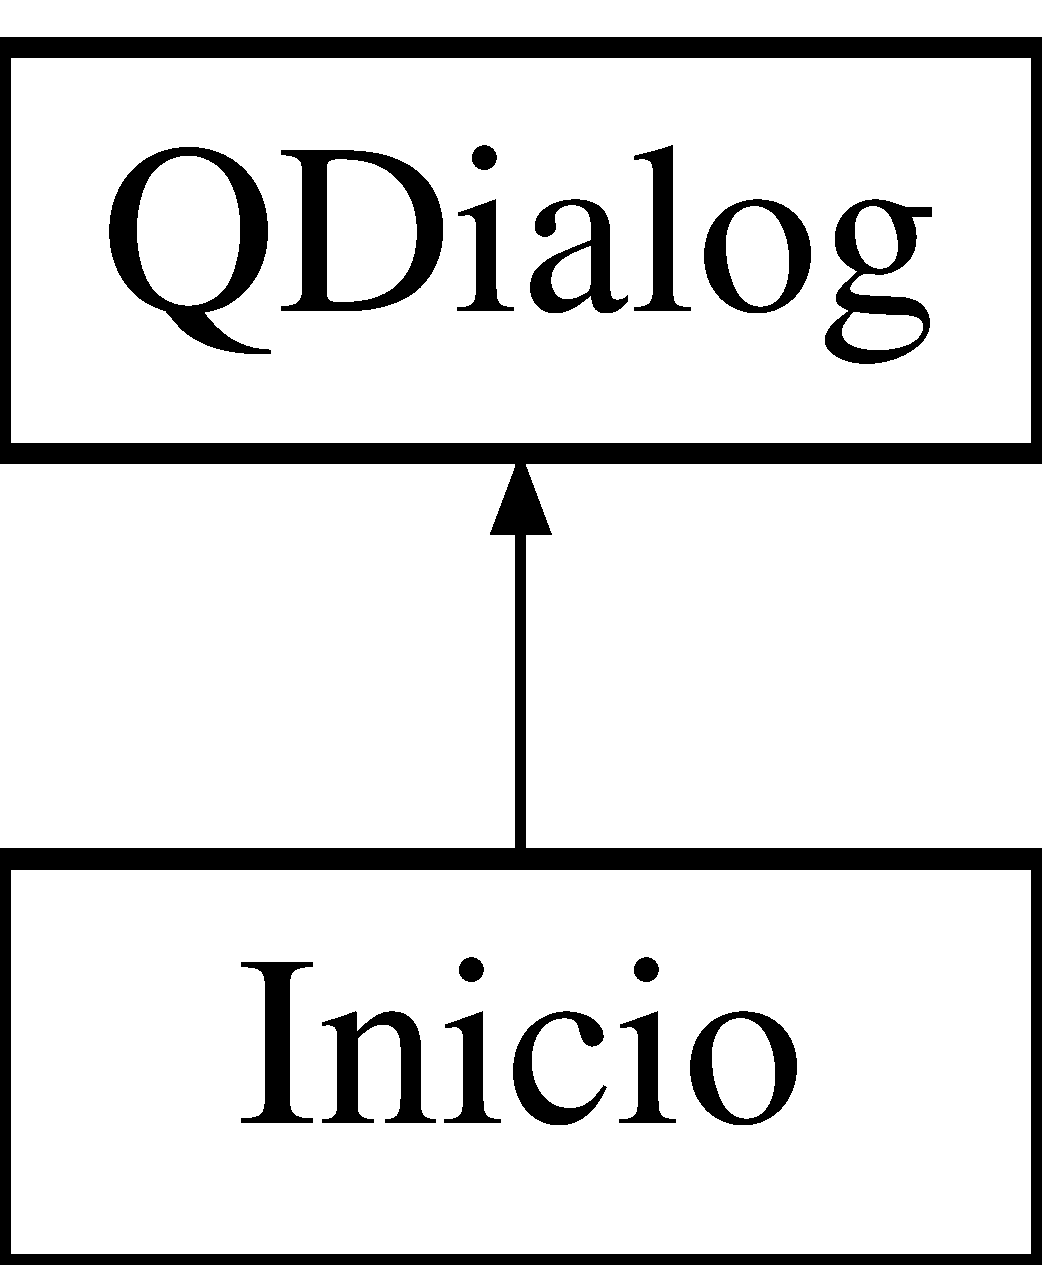
\includegraphics[height=2.000000cm]{class_inicio}
\end{center}
\end{figure}
\subsection*{Public Member Functions}
\begin{DoxyCompactItemize}
\item 
\hyperlink{class_inicio_aacdae4e557f144a4a3d664920ab8f1fa}{Inicio} (Q\-Widget $\ast$parent=0)
\end{DoxyCompactItemize}


\subsection{Constructor \& Destructor Documentation}
\hypertarget{class_inicio_aacdae4e557f144a4a3d664920ab8f1fa}{\index{Inicio@{Inicio}!Inicio@{Inicio}}
\index{Inicio@{Inicio}!Inicio@{Inicio}}
\subsubsection[{Inicio}]{\setlength{\rightskip}{0pt plus 5cm}Inicio\-::\-Inicio (
\begin{DoxyParamCaption}
\item[{Q\-Widget $\ast$}]{parent = {\ttfamily 0}}
\end{DoxyParamCaption}
)\hspace{0.3cm}{\ttfamily [explicit]}}}\label{class_inicio_aacdae4e557f144a4a3d664920ab8f1fa}
constructor de la clase inicio \begin{DoxyAuthor}{Author}
Kevin Campuzano
\end{DoxyAuthor}


The documentation for this class was generated from the following files\-:\begin{DoxyCompactItemize}
\item 
C\-:/\-Users/\-Janet/\-Documents/\-Git\-Hub/\-Final/\-Sudoku/inicio.\-h\item 
C\-:/\-Users/\-Janet/\-Documents/\-Git\-Hub/\-Final/\-Sudoku/inicio.\-cpp\end{DoxyCompactItemize}

\hypertarget{class_ui_1_1_inicio}{\section{Ui\-:\-:Inicio Class Reference}
\label{class_ui_1_1_inicio}\index{Ui\-::\-Inicio@{Ui\-::\-Inicio}}
}
Inheritance diagram for Ui\-:\-:Inicio\-:\begin{figure}[H]
\begin{center}
\leavevmode
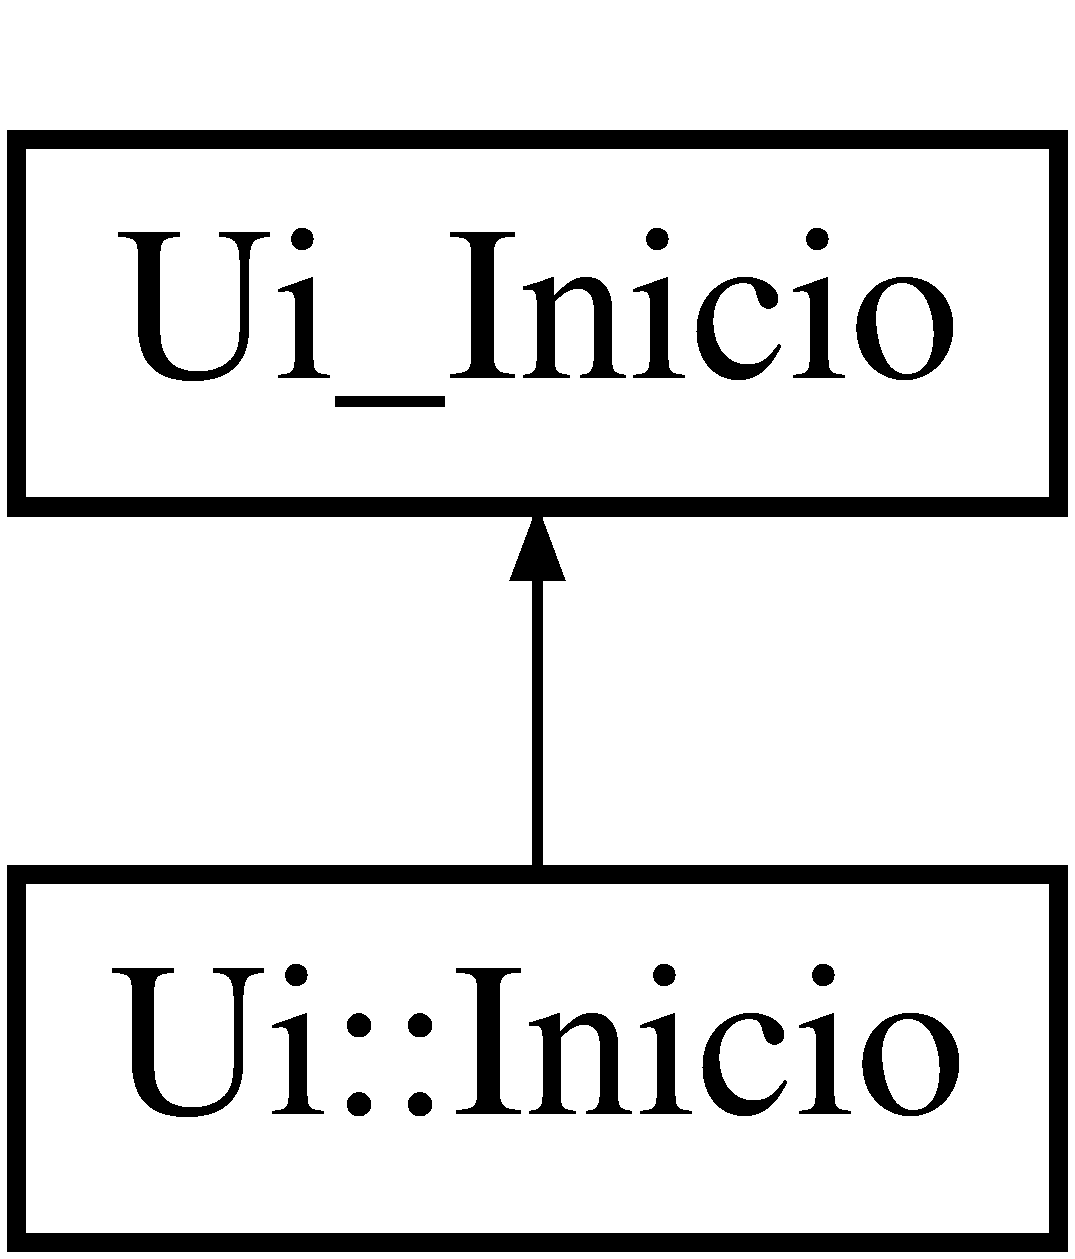
\includegraphics[height=2.000000cm]{class_ui_1_1_inicio}
\end{center}
\end{figure}
\subsection*{Additional Inherited Members}


The documentation for this class was generated from the following file\-:\begin{DoxyCompactItemize}
\item 
C\-:/\-Users/\-Janet/\-Documents/\-Git\-Hub/\-Final/build-\/\-Sudoku-\/\-Desktop\-\_\-\-Qt\-\_\-5\-\_\-0\-\_\-2\-\_\-\-Min\-G\-W\-\_\-32bit-\/\-Debug/ui\-\_\-inicio.\-h\end{DoxyCompactItemize}

\hypertarget{class_main_window}{\section{Main\-Window Class Reference}
\label{class_main_window}\index{Main\-Window@{Main\-Window}}
}
Inheritance diagram for Main\-Window\-:\begin{figure}[H]
\begin{center}
\leavevmode
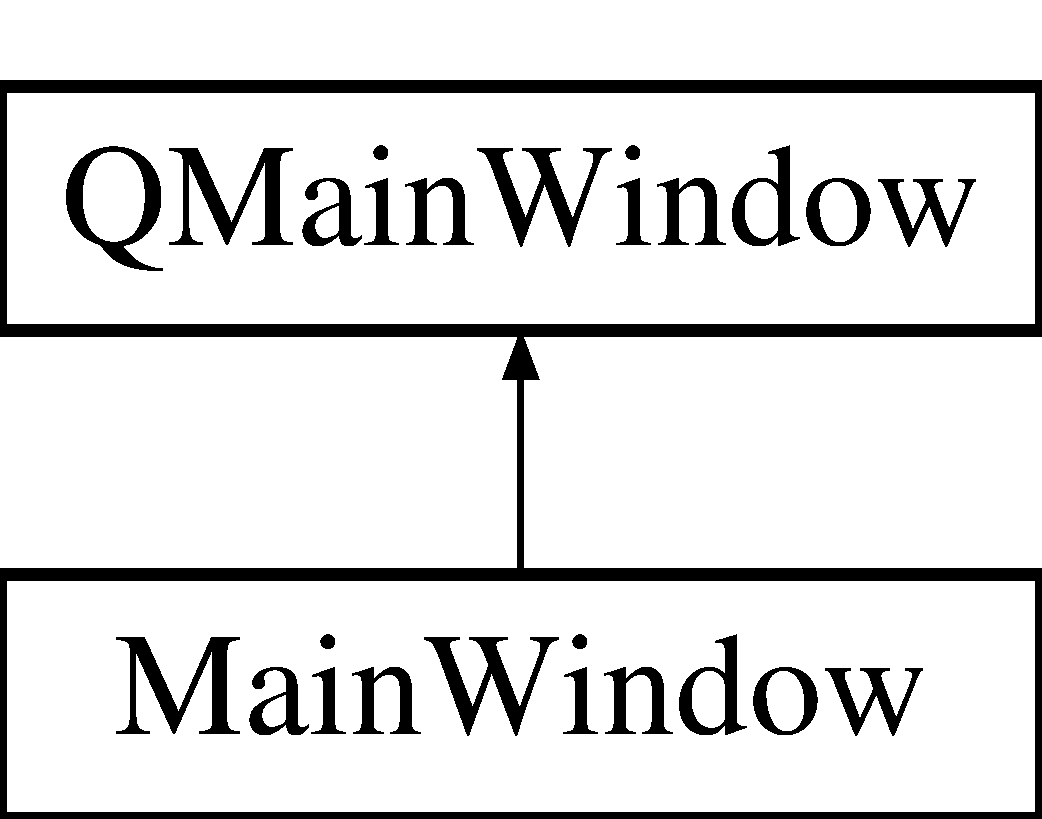
\includegraphics[height=2.000000cm]{class_main_window}
\end{center}
\end{figure}
\subsection*{Public Member Functions}
\begin{DoxyCompactItemize}
\item 
\hyperlink{class_main_window_a8b244be8b7b7db1b08de2a2acb9409db}{Main\-Window} (Q\-Widget $\ast$parent=0)
\item 
\hyperlink{class_main_window_ae98d00a93bc118200eeef9f9bba1dba7}{$\sim$\-Main\-Window} ()
\item 
void \hyperlink{class_main_window_a6f7ff976be1a9adfa19b23867f9c6d41}{load\-L\-E} (int dificultad, Q\-String nombre)
\item 
void \hyperlink{class_main_window_ab98df46367b9911377d5a85a293ae45f}{Comienza\-Cronometro} ()
\item 
void \hyperlink{class_main_window_a60f775aea4d2d76a37034f9659da20ff}{pintar} (list$<$ \hyperlink{class_cell}{Cell} $>$ e)
\item 
void \hyperlink{class_main_window_a4bba8622e7fca1f85bbb18e1eee37d71}{pintar\-Cell} (int x, int y, Q\-Color c)
\end{DoxyCompactItemize}
\subsection*{Public Attributes}
\begin{DoxyCompactItemize}
\item 
\hypertarget{class_main_window_a3584521b6f79321999e1c1613d5deedb}{\hyperlink{class_sudoku}{Sudoku} {\bfseries tablero}}\label{class_main_window_a3584521b6f79321999e1c1613d5deedb}

\item 
\hypertarget{class_main_window_ab06c0abc0234fe04c3d6720dd4bd71c2}{\hyperlink{class_sudoku}{Sudoku} {\bfseries juego}}\label{class_main_window_ab06c0abc0234fe04c3d6720dd4bd71c2}

\item 
\hypertarget{class_main_window_a5f9f0c071c52ca968564c2dc0210cf32}{\hyperlink{class_sudoku_generator}{Sudoku\-Generator} {\bfseries generator}}\label{class_main_window_a5f9f0c071c52ca968564c2dc0210cf32}

\end{DoxyCompactItemize}


\subsection{Constructor \& Destructor Documentation}
\hypertarget{class_main_window_a8b244be8b7b7db1b08de2a2acb9409db}{\index{Main\-Window@{Main\-Window}!Main\-Window@{Main\-Window}}
\index{Main\-Window@{Main\-Window}!MainWindow@{Main\-Window}}
\subsubsection[{Main\-Window}]{\setlength{\rightskip}{0pt plus 5cm}Main\-Window\-::\-Main\-Window (
\begin{DoxyParamCaption}
\item[{Q\-Widget $\ast$}]{parent = {\ttfamily 0}}
\end{DoxyParamCaption}
)\hspace{0.3cm}{\ttfamily [explicit]}}}\label{class_main_window_a8b244be8b7b7db1b08de2a2acb9409db}
constructor de la clase mainwindow \begin{DoxyAuthor}{Author}
Kevin Campuzano, Iván Aveiga
\end{DoxyAuthor}
\hypertarget{class_main_window_ae98d00a93bc118200eeef9f9bba1dba7}{\index{Main\-Window@{Main\-Window}!$\sim$\-Main\-Window@{$\sim$\-Main\-Window}}
\index{$\sim$\-Main\-Window@{$\sim$\-Main\-Window}!MainWindow@{Main\-Window}}
\subsubsection[{$\sim$\-Main\-Window}]{\setlength{\rightskip}{0pt plus 5cm}Main\-Window\-::$\sim$\-Main\-Window (
\begin{DoxyParamCaption}
{}
\end{DoxyParamCaption}
)}}\label{class_main_window_ae98d00a93bc118200eeef9f9bba1dba7}
Destructor de la clase mainwindow \begin{DoxyAuthor}{Author}
Qt
\end{DoxyAuthor}


\subsection{Member Function Documentation}
\hypertarget{class_main_window_ab98df46367b9911377d5a85a293ae45f}{\index{Main\-Window@{Main\-Window}!Comienza\-Cronometro@{Comienza\-Cronometro}}
\index{Comienza\-Cronometro@{Comienza\-Cronometro}!MainWindow@{Main\-Window}}
\subsubsection[{Comienza\-Cronometro}]{\setlength{\rightskip}{0pt plus 5cm}void Main\-Window\-::\-Comienza\-Cronometro (
\begin{DoxyParamCaption}
{}
\end{DoxyParamCaption}
)}}\label{class_main_window_ab98df46367b9911377d5a85a293ae45f}
inicia el cronómetro desde que es llamado el formulario mainwindow \begin{DoxyAuthor}{Author}
Kevin Campuzano
\end{DoxyAuthor}
\hypertarget{class_main_window_a6f7ff976be1a9adfa19b23867f9c6d41}{\index{Main\-Window@{Main\-Window}!load\-L\-E@{load\-L\-E}}
\index{load\-L\-E@{load\-L\-E}!MainWindow@{Main\-Window}}
\subsubsection[{load\-L\-E}]{\setlength{\rightskip}{0pt plus 5cm}void Main\-Window\-::load\-L\-E (
\begin{DoxyParamCaption}
\item[{int}]{dificultad, }
\item[{Q\-String}]{nombre}
\end{DoxyParamCaption}
)}}\label{class_main_window_a6f7ff976be1a9adfa19b23867f9c6d41}
carga en la interfaz el tablero a jugar con las celdas y el nombre del jugador. 
\begin{DoxyParams}{Parameters}
{\em dificultad,dificultad} & a jugar.  nombre, nombre del jugador. \\
\hline
\end{DoxyParams}
\begin{DoxyAuthor}{Author}
Iván Aveiga
\end{DoxyAuthor}
\hypertarget{class_main_window_a60f775aea4d2d76a37034f9659da20ff}{\index{Main\-Window@{Main\-Window}!pintar@{pintar}}
\index{pintar@{pintar}!MainWindow@{Main\-Window}}
\subsubsection[{pintar}]{\setlength{\rightskip}{0pt plus 5cm}void Main\-Window\-::pintar (
\begin{DoxyParamCaption}
\item[{list$<$ {\bf Cell} $>$}]{e}
\end{DoxyParamCaption}
)}}\label{class_main_window_a60f775aea4d2d76a37034f9659da20ff}
Pinta las celdas erróneas 
\begin{DoxyParams}{Parameters}
{\em e} & lista de celdas erróneas. \\
\hline
\end{DoxyParams}
\begin{DoxyAuthor}{Author}
Ivan Aveiga
\end{DoxyAuthor}
\hypertarget{class_main_window_a4bba8622e7fca1f85bbb18e1eee37d71}{\index{Main\-Window@{Main\-Window}!pintar\-Cell@{pintar\-Cell}}
\index{pintar\-Cell@{pintar\-Cell}!MainWindow@{Main\-Window}}
\subsubsection[{pintar\-Cell}]{\setlength{\rightskip}{0pt plus 5cm}void Main\-Window\-::pintar\-Cell (
\begin{DoxyParamCaption}
\item[{int}]{x, }
\item[{int}]{y, }
\item[{Q\-Color}]{c}
\end{DoxyParamCaption}
)}}\label{class_main_window_a4bba8622e7fca1f85bbb18e1eee37d71}
Pinta una celda de color 
\begin{DoxyParams}{Parameters}
{\em x} & coordenada en x de la celda \\
\hline
{\em y} & coordenada en y de la celda  color ha ser pintado.\\
\hline
\end{DoxyParams}


The documentation for this class was generated from the following files\-:\begin{DoxyCompactItemize}
\item 
C\-:/\-Users/\-Janet/\-Documents/\-Git\-Hub/\-Final/\-Sudoku/mainwindow.\-h\item 
C\-:/\-Users/\-Janet/\-Documents/\-Git\-Hub/\-Final/\-Sudoku/mainwindow.\-cpp\end{DoxyCompactItemize}

\hypertarget{class_ui_1_1_main_window}{\section{Ui\-:\-:Main\-Window Class Reference}
\label{class_ui_1_1_main_window}\index{Ui\-::\-Main\-Window@{Ui\-::\-Main\-Window}}
}
Inheritance diagram for Ui\-:\-:Main\-Window\-:\begin{figure}[H]
\begin{center}
\leavevmode
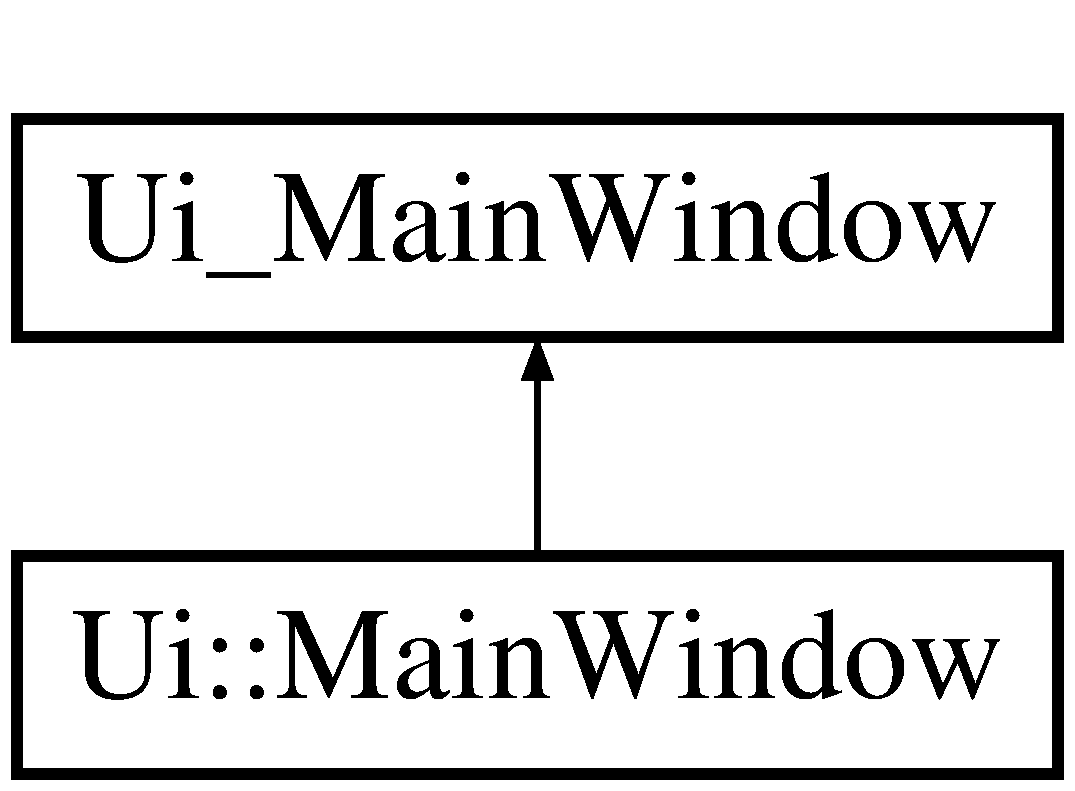
\includegraphics[height=2.000000cm]{class_ui_1_1_main_window}
\end{center}
\end{figure}
\subsection*{Additional Inherited Members}


The documentation for this class was generated from the following file\-:\begin{DoxyCompactItemize}
\item 
C\-:/\-Users/\-Janet/\-Documents/\-Git\-Hub/\-Final/build-\/\-Sudoku-\/\-Desktop\-\_\-\-Qt\-\_\-5\-\_\-0\-\_\-2\-\_\-\-Min\-G\-W\-\_\-32bit-\/\-Debug/ui\-\_\-mainwindow.\-h\end{DoxyCompactItemize}

\hypertarget{structqt__meta__stringdata___inicio__t}{\section{qt\-\_\-meta\-\_\-stringdata\-\_\-\-Inicio\-\_\-t Struct Reference}
\label{structqt__meta__stringdata___inicio__t}\index{qt\-\_\-meta\-\_\-stringdata\-\_\-\-Inicio\-\_\-t@{qt\-\_\-meta\-\_\-stringdata\-\_\-\-Inicio\-\_\-t}}
}
\subsection*{Public Attributes}
\begin{DoxyCompactItemize}
\item 
\hypertarget{structqt__meta__stringdata___inicio__t_a8523396fd1dfbb6099467bf7c19f37fc}{Q\-Byte\-Array\-Data {\bfseries data} \mbox{[}4\mbox{]}}\label{structqt__meta__stringdata___inicio__t_a8523396fd1dfbb6099467bf7c19f37fc}

\item 
\hypertarget{structqt__meta__stringdata___inicio__t_ae3d2ecd95c9ddaf94f6cc7efb002f617}{char {\bfseries stringdata} \mbox{[}35\mbox{]}}\label{structqt__meta__stringdata___inicio__t_ae3d2ecd95c9ddaf94f6cc7efb002f617}

\end{DoxyCompactItemize}


The documentation for this struct was generated from the following file\-:\begin{DoxyCompactItemize}
\item 
C\-:/\-Users/\-Janet/\-Documents/\-Git\-Hub/\-Final/build-\/\-Sudoku-\/\-Desktop\-\_\-\-Qt\-\_\-5\-\_\-0\-\_\-2\-\_\-\-Min\-G\-W\-\_\-32bit-\/\-Debug/debug/moc\-\_\-inicio.\-cpp\end{DoxyCompactItemize}

\hypertarget{structqt__meta__stringdata___main_window__t}{\section{qt\-\_\-meta\-\_\-stringdata\-\_\-\-Main\-Window\-\_\-t Struct Reference}
\label{structqt__meta__stringdata___main_window__t}\index{qt\-\_\-meta\-\_\-stringdata\-\_\-\-Main\-Window\-\_\-t@{qt\-\_\-meta\-\_\-stringdata\-\_\-\-Main\-Window\-\_\-t}}
}
\subsection*{Public Attributes}
\begin{DoxyCompactItemize}
\item 
\hypertarget{structqt__meta__stringdata___main_window__t_a728217305ebd7d8895235c2038c4ed28}{Q\-Byte\-Array\-Data {\bfseries data} \mbox{[}5\mbox{]}}\label{structqt__meta__stringdata___main_window__t_a728217305ebd7d8895235c2038c4ed28}

\item 
\hypertarget{structqt__meta__stringdata___main_window__t_a308c2ea0257b1ad83ad81c262035d8a6}{char {\bfseries stringdata} \mbox{[}43\mbox{]}}\label{structqt__meta__stringdata___main_window__t_a308c2ea0257b1ad83ad81c262035d8a6}

\end{DoxyCompactItemize}


The documentation for this struct was generated from the following file\-:\begin{DoxyCompactItemize}
\item 
C\-:/\-Users/\-Janet/\-Documents/\-Git\-Hub/\-Final/build-\/\-Sudoku-\/\-Desktop\-\_\-\-Qt\-\_\-5\-\_\-0\-\_\-2\-\_\-\-Min\-G\-W\-\_\-32bit-\/\-Debug/debug/moc\-\_\-mainwindow.\-cpp\end{DoxyCompactItemize}

\hypertarget{class_sudoku}{\section{Sudoku Class Reference}
\label{class_sudoku}\index{Sudoku@{Sudoku}}
}
\subsection*{Public Member Functions}
\begin{DoxyCompactItemize}
\item 
\hyperlink{class_sudoku_a5fc6547fe577e8eca24a7e86d2fa0ff8}{Sudoku} ()
\item 
void \hyperlink{class_sudoku_adc8056faf07d87de883a158b725e6147}{set\-Cell} (int i, int j, \hyperlink{class_cell}{Cell} c)
\begin{DoxyCompactList}\small\item\em Ingresa la celda c en la posición ij. \end{DoxyCompactList}\item 
\hyperlink{class_cell}{Cell} \hyperlink{class_sudoku_aedf7e9b2aff39c2c7780f3d86d2cce4a}{get\-Cell} (int i, int j)
\begin{DoxyCompactList}\small\item\em Ingresa la posicion y devuelve la celda. \end{DoxyCompactList}\item 
double \hyperlink{class_sudoku_abd9fe1e98fac81bcc091efad36471aee}{distance} (\hyperlink{class_cell}{Cell} c, \hyperlink{class_cell}{Cell} d)
\begin{DoxyCompactList}\small\item\em Calcula la distancia que hay de una celda a otra. \end{DoxyCompactList}\item 
void \hyperlink{class_sudoku_a924e2ea0f124bf62dab548fbc3874306}{load\-Sudoku} ()
\item 
\hyperlink{class_cell}{Cell} \hyperlink{class_sudoku_ae93e04817312534e48406d7fc5c56613}{get\-Center} (\hyperlink{class_cell}{Cell} c)
\item 
void \hyperlink{class_sudoku_a0929ca2fcbf280b6a769917791ca8406}{initialize\-Centers} ()
\item 
list$<$ \hyperlink{class_cell}{Cell} $>$ \hyperlink{class_sudoku_af8ca2a52ac9f9385aa581e188600d313}{check\-Col} (\hyperlink{class_cell}{Cell} c)
\item 
list$<$ \hyperlink{class_cell}{Cell} $>$ \hyperlink{class_sudoku_a827821ce9fdcacfe62f3986cd9be9db1}{check\-Row} (\hyperlink{class_cell}{Cell} c)
\item 
bool \hyperlink{class_sudoku_a057dd2f4b6987c0d13a230ed9ea3a347}{in\-List} (list$<$ \hyperlink{class_cell}{Cell} $>$ a, \hyperlink{class_cell}{Cell} b)
\item 
\hypertarget{class_sudoku_a2577a9930026b4b3ab85fe72175fb5e0}{list$<$ \hyperlink{class_cell}{Cell} $>$ {\bfseries merge\-Lists} (list$<$ \hyperlink{class_cell}{Cell} $>$ A, list$<$ \hyperlink{class_cell}{Cell} $>$ B)}\label{class_sudoku_a2577a9930026b4b3ab85fe72175fb5e0}

\item 
\hypertarget{class_sudoku_ab4b45a515f86cc6e4c69697e1e18d939}{list$<$ \hyperlink{class_cell}{Cell} $>$ {\bfseries check\-Submatrix} (\hyperlink{class_cell}{Cell} c)}\label{class_sudoku_ab4b45a515f86cc6e4c69697e1e18d939}

\item 
list$<$ \hyperlink{class_cell}{Cell} $>$ \hyperlink{class_sudoku_a4e2df01814bbe166489cad8819c5b516}{check\-All} ()
\item 
list$<$ \hyperlink{class_cell}{Cell} $>$ \hyperlink{class_sudoku_a01c67f46dda4d8885196a841ef5b4519}{compare} (\hyperlink{class_sudoku}{Sudoku} t)
\item 
bool \hyperlink{class_sudoku_a50853e36aa47d55769d91f7dfe318c94}{is\-Valid} ()
\end{DoxyCompactItemize}


\subsection{Constructor \& Destructor Documentation}
\hypertarget{class_sudoku_a5fc6547fe577e8eca24a7e86d2fa0ff8}{\index{Sudoku@{Sudoku}!Sudoku@{Sudoku}}
\index{Sudoku@{Sudoku}!Sudoku@{Sudoku}}
\subsubsection[{Sudoku}]{\setlength{\rightskip}{0pt plus 5cm}Sudoku\-::\-Sudoku (
\begin{DoxyParamCaption}
{}
\end{DoxyParamCaption}
)}}\label{class_sudoku_a5fc6547fe577e8eca24a7e86d2fa0ff8}
Constructor de la clase \hyperlink{class_sudoku}{Sudoku}, las celdas se inicializan con un valor de 0. \begin{DoxyAuthor}{Author}
Iván Aveiga.
\end{DoxyAuthor}


\subsection{Member Function Documentation}
\hypertarget{class_sudoku_a4e2df01814bbe166489cad8819c5b516}{\index{Sudoku@{Sudoku}!check\-All@{check\-All}}
\index{check\-All@{check\-All}!Sudoku@{Sudoku}}
\subsubsection[{check\-All}]{\setlength{\rightskip}{0pt plus 5cm}list$<$ {\bf Cell} $>$ Sudoku\-::check\-All (
\begin{DoxyParamCaption}
{}
\end{DoxyParamCaption}
)}}\label{class_sudoku_a4e2df01814bbe166489cad8819c5b516}
retorna todas las celdas conflictivas de un tablero de sudoku \begin{DoxyReturn}{Returns}
lista de celdas conflictivas 
\end{DoxyReturn}
\begin{DoxyAuthor}{Author}
Iván Aveiga Based in an idea of Nathalie Tejena.
\end{DoxyAuthor}
\hypertarget{class_sudoku_af8ca2a52ac9f9385aa581e188600d313}{\index{Sudoku@{Sudoku}!check\-Col@{check\-Col}}
\index{check\-Col@{check\-Col}!Sudoku@{Sudoku}}
\subsubsection[{check\-Col}]{\setlength{\rightskip}{0pt plus 5cm}list$<$ {\bf Cell} $>$ Sudoku\-::check\-Col (
\begin{DoxyParamCaption}
\item[{{\bf Cell}}]{c}
\end{DoxyParamCaption}
)}}\label{class_sudoku_af8ca2a52ac9f9385aa581e188600d313}
Retorna las celdas repetidas en la fila de c. 
\begin{DoxyParams}{Parameters}
{\em c} & Celda a buscar en la filaa c.\-x. \\
\hline
\end{DoxyParams}
\begin{DoxyReturn}{Returns}
lista de celdas repetidas a c. 
\end{DoxyReturn}
\begin{DoxyAuthor}{Author}
Iván Aveiga
\end{DoxyAuthor}
\hypertarget{class_sudoku_a827821ce9fdcacfe62f3986cd9be9db1}{\index{Sudoku@{Sudoku}!check\-Row@{check\-Row}}
\index{check\-Row@{check\-Row}!Sudoku@{Sudoku}}
\subsubsection[{check\-Row}]{\setlength{\rightskip}{0pt plus 5cm}list$<$ {\bf Cell} $>$ Sudoku\-::check\-Row (
\begin{DoxyParamCaption}
\item[{{\bf Cell}}]{c}
\end{DoxyParamCaption}
)}}\label{class_sudoku_a827821ce9fdcacfe62f3986cd9be9db1}
Retorna las celdas repetidas en la columna de c. 
\begin{DoxyParams}{Parameters}
{\em c} & Celda a buscar en la columna c.\-y. \\
\hline
\end{DoxyParams}
\begin{DoxyReturn}{Returns}
lista de celdas repetidas a c. 
\end{DoxyReturn}
\begin{DoxyAuthor}{Author}
Iván Aveiga
\end{DoxyAuthor}
\hypertarget{class_sudoku_a01c67f46dda4d8885196a841ef5b4519}{\index{Sudoku@{Sudoku}!compare@{compare}}
\index{compare@{compare}!Sudoku@{Sudoku}}
\subsubsection[{compare}]{\setlength{\rightskip}{0pt plus 5cm}list$<$ {\bf Cell} $>$ Sudoku\-::compare (
\begin{DoxyParamCaption}
\item[{{\bf Sudoku}}]{t}
\end{DoxyParamCaption}
)}}\label{class_sudoku_a01c67f46dda4d8885196a841ef5b4519}
Compara dos sudokus y devuelve la lista de celdas distintas del sudoku. 
\begin{DoxyParams}{Parameters}
{\em t} & \hyperlink{class_sudoku}{Sudoku} que servirá como base a comparar celdas (\hyperlink{class_cell}{Cell}). \\
\hline
\end{DoxyParams}
\begin{DoxyReturn}{Returns}
la lista de celdas que no coinciden entre this y t, tomando como base t. 
\end{DoxyReturn}
\begin{DoxyAuthor}{Author}
Iván Aveiga
\end{DoxyAuthor}
\hypertarget{class_sudoku_abd9fe1e98fac81bcc091efad36471aee}{\index{Sudoku@{Sudoku}!distance@{distance}}
\index{distance@{distance}!Sudoku@{Sudoku}}
\subsubsection[{distance}]{\setlength{\rightskip}{0pt plus 5cm}double Sudoku\-::distance (
\begin{DoxyParamCaption}
\item[{{\bf Cell}}]{c, }
\item[{{\bf Cell}}]{d}
\end{DoxyParamCaption}
)}}\label{class_sudoku_abd9fe1e98fac81bcc091efad36471aee}


Calcula la distancia que hay de una celda a otra. 


\begin{DoxyParams}{Parameters}
{\em c} & celda inicial. \\
\hline
{\em d} & celda final. \\
\hline
\end{DoxyParams}
\begin{DoxyReturn}{Returns}
distancia de una celda a otra. 
\end{DoxyReturn}
\begin{DoxyAuthor}{Author}
Iván Aveiga. 
\end{DoxyAuthor}
\hypertarget{class_sudoku_aedf7e9b2aff39c2c7780f3d86d2cce4a}{\index{Sudoku@{Sudoku}!get\-Cell@{get\-Cell}}
\index{get\-Cell@{get\-Cell}!Sudoku@{Sudoku}}
\subsubsection[{get\-Cell}]{\setlength{\rightskip}{0pt plus 5cm}{\bf Cell} Sudoku\-::get\-Cell (
\begin{DoxyParamCaption}
\item[{int}]{i, }
\item[{int}]{j}
\end{DoxyParamCaption}
)}}\label{class_sudoku_aedf7e9b2aff39c2c7780f3d86d2cce4a}


Ingresa la posicion y devuelve la celda. 


\begin{DoxyParams}{Parameters}
{\em i} & posicion de la celda en x(columna). \\
\hline
{\em j} & posicion de la celda en y(fila). \\
\hline
\end{DoxyParams}
\begin{DoxyReturn}{Returns}
retorna la celda ij de la matriz. 
\end{DoxyReturn}
\begin{DoxyAuthor}{Author}
Iván Aveiga. 
\end{DoxyAuthor}
\hypertarget{class_sudoku_ae93e04817312534e48406d7fc5c56613}{\index{Sudoku@{Sudoku}!get\-Center@{get\-Center}}
\index{get\-Center@{get\-Center}!Sudoku@{Sudoku}}
\subsubsection[{get\-Center}]{\setlength{\rightskip}{0pt plus 5cm}{\bf Cell} Sudoku\-::get\-Center (
\begin{DoxyParamCaption}
\item[{{\bf Cell}}]{c}
\end{DoxyParamCaption}
)}}\label{class_sudoku_ae93e04817312534e48406d7fc5c56613}
obtiene la celda central de la submatriz perteneciente a c. 
\begin{DoxyParams}{Parameters}
{\em c} & Celda a calcular a que submatriz pertenece. \\
\hline
\end{DoxyParams}
\begin{DoxyReturn}{Returns}
retorna celda central correspondiente a la submatriz donde c pertenece. 
\end{DoxyReturn}
\begin{DoxyAuthor}{Author}
Iván Aveiga
\end{DoxyAuthor}
\hypertarget{class_sudoku_a0929ca2fcbf280b6a769917791ca8406}{\index{Sudoku@{Sudoku}!initialize\-Centers@{initialize\-Centers}}
\index{initialize\-Centers@{initialize\-Centers}!Sudoku@{Sudoku}}
\subsubsection[{initialize\-Centers}]{\setlength{\rightskip}{0pt plus 5cm}void Sudoku\-::initialize\-Centers (
\begin{DoxyParamCaption}
{}
\end{DoxyParamCaption}
)}}\label{class_sudoku_a0929ca2fcbf280b6a769917791ca8406}
Inicializa el vector de centros para determinar a que submatriz pertenece una celda \begin{DoxyAuthor}{Author}
Iván Aveiga
\end{DoxyAuthor}
\hypertarget{class_sudoku_a057dd2f4b6987c0d13a230ed9ea3a347}{\index{Sudoku@{Sudoku}!in\-List@{in\-List}}
\index{in\-List@{in\-List}!Sudoku@{Sudoku}}
\subsubsection[{in\-List}]{\setlength{\rightskip}{0pt plus 5cm}bool Sudoku\-::in\-List (
\begin{DoxyParamCaption}
\item[{list$<$ {\bf Cell} $>$}]{a, }
\item[{{\bf Cell}}]{b}
\end{DoxyParamCaption}
)}}\label{class_sudoku_a057dd2f4b6987c0d13a230ed9ea3a347}
Devuelve verdadero si la celda b se encuentra en la lista de celdas a. 
\begin{DoxyParams}{Parameters}
{\em a} & \-: Lista de Celdas. \\
\hline
{\em b} & \-: Celda a buscar si se encuentra en a. \\
\hline
\end{DoxyParams}
\begin{DoxyReturn}{Returns}
un valor booleano dependiendo si se encuentra o no b en a. 
\end{DoxyReturn}
\begin{DoxyAuthor}{Author}
Iván Aveiga.
\end{DoxyAuthor}
\hypertarget{class_sudoku_a50853e36aa47d55769d91f7dfe318c94}{\index{Sudoku@{Sudoku}!is\-Valid@{is\-Valid}}
\index{is\-Valid@{is\-Valid}!Sudoku@{Sudoku}}
\subsubsection[{is\-Valid}]{\setlength{\rightskip}{0pt plus 5cm}bool Sudoku\-::is\-Valid (
\begin{DoxyParamCaption}
{}
\end{DoxyParamCaption}
)}}\label{class_sudoku_a50853e36aa47d55769d91f7dfe318c94}
Retorna verdadero si un tablero \hyperlink{class_sudoku}{Sudoku} es válido, falso si es inválido. \begin{DoxyReturn}{Returns}
Un valor booleano. 
\end{DoxyReturn}
\begin{DoxyAuthor}{Author}
Iván Aveiga
\end{DoxyAuthor}
\hypertarget{class_sudoku_a924e2ea0f124bf62dab548fbc3874306}{\index{Sudoku@{Sudoku}!load\-Sudoku@{load\-Sudoku}}
\index{load\-Sudoku@{load\-Sudoku}!Sudoku@{Sudoku}}
\subsubsection[{load\-Sudoku}]{\setlength{\rightskip}{0pt plus 5cm}void Sudoku\-::load\-Sudoku (
\begin{DoxyParamCaption}
{}
\end{DoxyParamCaption}
)}}\label{class_sudoku_a924e2ea0f124bf62dab548fbc3874306}
Carga un sudoku aleatorio de un archivo de texto plano. \begin{DoxyAuthor}{Author}
Iván Aveiga
\end{DoxyAuthor}
\hypertarget{class_sudoku_adc8056faf07d87de883a158b725e6147}{\index{Sudoku@{Sudoku}!set\-Cell@{set\-Cell}}
\index{set\-Cell@{set\-Cell}!Sudoku@{Sudoku}}
\subsubsection[{set\-Cell}]{\setlength{\rightskip}{0pt plus 5cm}void Sudoku\-::set\-Cell (
\begin{DoxyParamCaption}
\item[{int}]{i, }
\item[{int}]{j, }
\item[{{\bf Cell}}]{c}
\end{DoxyParamCaption}
)}}\label{class_sudoku_adc8056faf07d87de883a158b725e6147}


Ingresa la celda c en la posición ij. 


\begin{DoxyParams}{Parameters}
{\em i} & posicion de la celda en x(fila) \\
\hline
{\em j} & posicion de la celda en y(columna) \\
\hline
{\em c} & celda a ser almacenada en la posición ij \\
\hline
\end{DoxyParams}
\begin{DoxyAuthor}{Author}
Iván Aveiga 
\end{DoxyAuthor}


The documentation for this class was generated from the following files\-:\begin{DoxyCompactItemize}
\item 
C\-:/\-Users/\-Janet/\-Documents/\-Git\-Hub/\-Final/\-Sudoku/sudoku.\-h\item 
C\-:/\-Users/\-Janet/\-Documents/\-Git\-Hub/\-Final/\-Sudoku/sudoku.\-cpp\end{DoxyCompactItemize}

\hypertarget{class_sudoku_generator}{\section{Sudoku\-Generator Class Reference}
\label{class_sudoku_generator}\index{Sudoku\-Generator@{Sudoku\-Generator}}
}
\subsection*{Public Member Functions}
\begin{DoxyCompactItemize}
\item 
\hyperlink{class_sudoku_generator_aa14a5aa7c33ccc472c6b1f4fd7714855}{Sudoku\-Generator} ()
\item 
\hyperlink{class_sudoku}{Sudoku} \hyperlink{class_sudoku_generator_a75a7326eff7423eae1ca25c5c473d89b}{get\-Board\-Game} ()
\item 
void \hyperlink{class_sudoku_generator_a0c02c1bd837e80d95a097a45a8d5b95d}{set\-Board\-Game} (\hyperlink{class_sudoku}{Sudoku} s)
\item 
\hyperlink{class_sudoku}{Sudoku} \hyperlink{class_sudoku_generator_a055eed3a39b7a54df1badee216abbca2}{generate} (\hyperlink{class_sudoku}{Sudoku} s, int dificulty)
\end{DoxyCompactItemize}


\subsection{Constructor \& Destructor Documentation}
\hypertarget{class_sudoku_generator_aa14a5aa7c33ccc472c6b1f4fd7714855}{\index{Sudoku\-Generator@{Sudoku\-Generator}!Sudoku\-Generator@{Sudoku\-Generator}}
\index{Sudoku\-Generator@{Sudoku\-Generator}!SudokuGenerator@{Sudoku\-Generator}}
\subsubsection[{Sudoku\-Generator}]{\setlength{\rightskip}{0pt plus 5cm}Sudoku\-Generator\-::\-Sudoku\-Generator (
\begin{DoxyParamCaption}
{}
\end{DoxyParamCaption}
)}}\label{class_sudoku_generator_aa14a5aa7c33ccc472c6b1f4fd7714855}
Crea un \hyperlink{class_sudoku_generator}{Sudoku\-Generator}. \begin{DoxyAuthor}{Author}
Iván Aveiga.
\end{DoxyAuthor}


\subsection{Member Function Documentation}
\hypertarget{class_sudoku_generator_a055eed3a39b7a54df1badee216abbca2}{\index{Sudoku\-Generator@{Sudoku\-Generator}!generate@{generate}}
\index{generate@{generate}!SudokuGenerator@{Sudoku\-Generator}}
\subsubsection[{generate}]{\setlength{\rightskip}{0pt plus 5cm}{\bf Sudoku} Sudoku\-Generator\-::generate (
\begin{DoxyParamCaption}
\item[{{\bf Sudoku}}]{s, }
\item[{int}]{dificulty}
\end{DoxyParamCaption}
)}}\label{class_sudoku_generator_a055eed3a39b7a54df1badee216abbca2}
Devuelve un sudoku para jugar según la dificultad. 
\begin{DoxyParams}{Parameters}
{\em s,sudoku} & del cuál se obtendrá las celdas para armar el sudoku. \\
\hline
{\em dificulty,dificultad} & para generar el tablero, se basa en las celdas a elegir \\
\hline
\end{DoxyParams}
\begin{DoxyReturn}{Returns}
un sudoku parcialmente completado para jugar. 
\end{DoxyReturn}
\begin{DoxyAuthor}{Author}
Iván Aveiga.
\end{DoxyAuthor}
Genera un tablero nuevo a partir de s, dificultades\-: 1\-: Fácil $|$ 41 -\/ 36 Fichas 2\-: Normal $|$ 35 -\/ 32 Fichas 3\-: Avanzado $|$ 31 -\/ 28 Fichas 4\-: Experto $|$ 27 -\/ 23 Fichas Obtenido de Programming \hyperlink{class_sudoku}{Sudoku}, Meng Lee.\hypertarget{class_sudoku_generator_a75a7326eff7423eae1ca25c5c473d89b}{\index{Sudoku\-Generator@{Sudoku\-Generator}!get\-Board\-Game@{get\-Board\-Game}}
\index{get\-Board\-Game@{get\-Board\-Game}!SudokuGenerator@{Sudoku\-Generator}}
\subsubsection[{get\-Board\-Game}]{\setlength{\rightskip}{0pt plus 5cm}{\bf Sudoku} Sudoku\-Generator\-::get\-Board\-Game (
\begin{DoxyParamCaption}
{}
\end{DoxyParamCaption}
)}}\label{class_sudoku_generator_a75a7326eff7423eae1ca25c5c473d89b}
Devuelve el atributo board\-Game. \begin{DoxyReturn}{Returns}
atributo board\-Game. 
\end{DoxyReturn}
\begin{DoxyAuthor}{Author}
Iván Aveiga.
\end{DoxyAuthor}
\hypertarget{class_sudoku_generator_a0c02c1bd837e80d95a097a45a8d5b95d}{\index{Sudoku\-Generator@{Sudoku\-Generator}!set\-Board\-Game@{set\-Board\-Game}}
\index{set\-Board\-Game@{set\-Board\-Game}!SudokuGenerator@{Sudoku\-Generator}}
\subsubsection[{set\-Board\-Game}]{\setlength{\rightskip}{0pt plus 5cm}void Sudoku\-Generator\-::set\-Board\-Game (
\begin{DoxyParamCaption}
\item[{{\bf Sudoku}}]{s}
\end{DoxyParamCaption}
)}}\label{class_sudoku_generator_a0c02c1bd837e80d95a097a45a8d5b95d}
Setea el atributo board\-Game con el sudoku s. 
\begin{DoxyParams}{Parameters}
{\em s,sudoku.} & \\
\hline
\end{DoxyParams}
\begin{DoxyAuthor}{Author}
Iván Aveiga.
\end{DoxyAuthor}


The documentation for this class was generated from the following files\-:\begin{DoxyCompactItemize}
\item 
C\-:/\-Users/\-Janet/\-Documents/\-Git\-Hub/\-Final/\-Sudoku/sudokugenerator.\-h\item 
C\-:/\-Users/\-Janet/\-Documents/\-Git\-Hub/\-Final/\-Sudoku/sudokugenerator.\-cpp\end{DoxyCompactItemize}

\hypertarget{class_ui___inicio}{\section{Ui\-\_\-\-Inicio Class Reference}
\label{class_ui___inicio}\index{Ui\-\_\-\-Inicio@{Ui\-\_\-\-Inicio}}
}
Inheritance diagram for Ui\-\_\-\-Inicio\-:\begin{figure}[H]
\begin{center}
\leavevmode
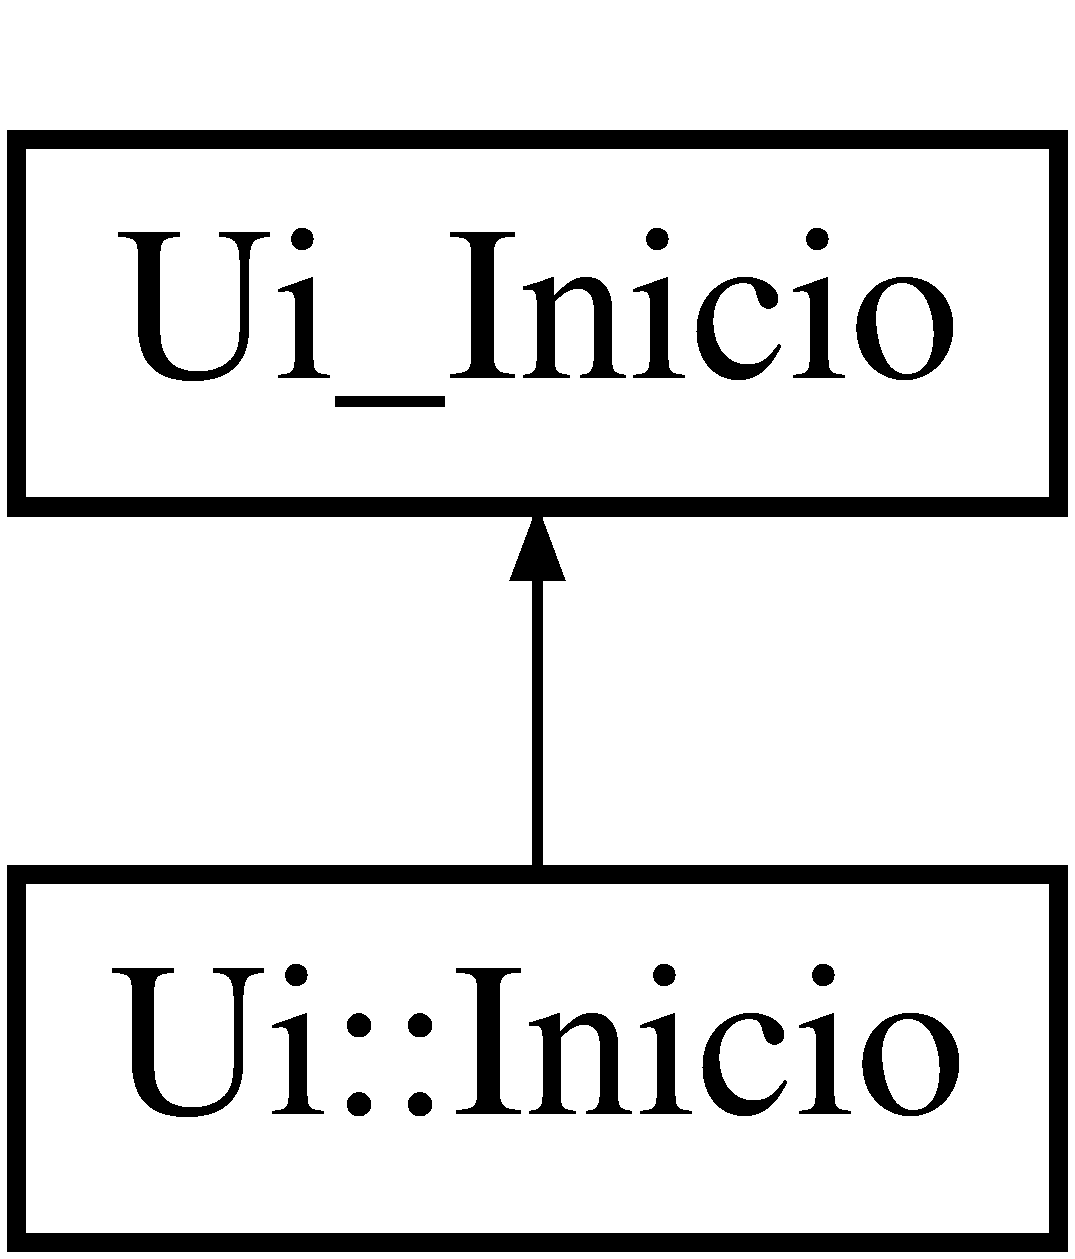
\includegraphics[height=2.000000cm]{class_ui___inicio}
\end{center}
\end{figure}
\subsection*{Public Member Functions}
\begin{DoxyCompactItemize}
\item 
\hypertarget{class_ui___inicio_a1688343a8860c7f725c89169263f0346}{void {\bfseries setup\-Ui} (Q\-Dialog $\ast$\hyperlink{class_inicio}{Inicio})}\label{class_ui___inicio_a1688343a8860c7f725c89169263f0346}

\item 
\hypertarget{class_ui___inicio_afb48f892cfc61a817b0363b692aef769}{void {\bfseries retranslate\-Ui} (Q\-Dialog $\ast$\hyperlink{class_inicio}{Inicio})}\label{class_ui___inicio_afb48f892cfc61a817b0363b692aef769}

\end{DoxyCompactItemize}
\subsection*{Public Attributes}
\begin{DoxyCompactItemize}
\item 
\hypertarget{class_ui___inicio_a361663afe17bec1307d987567c1ad8b3}{Q\-Push\-Button $\ast$ {\bfseries btn\-\_\-jugar}}\label{class_ui___inicio_a361663afe17bec1307d987567c1ad8b3}

\item 
\hypertarget{class_ui___inicio_aba8ea0f0be152b9fef6003c681fe30f1}{Q\-Push\-Button $\ast$ {\bfseries btn\-\_\-\-Salir}}\label{class_ui___inicio_aba8ea0f0be152b9fef6003c681fe30f1}

\item 
\hypertarget{class_ui___inicio_a2916bec7b4a674d6a123e468ee2a5d24}{Q\-Radio\-Button $\ast$ {\bfseries rbt\-\_\-facil}}\label{class_ui___inicio_a2916bec7b4a674d6a123e468ee2a5d24}

\item 
\hypertarget{class_ui___inicio_a8a2bc7dc7d0d8a833ebf39b0c7e17077}{Q\-Radio\-Button $\ast$ {\bfseries rbt\-\_\-normal}}\label{class_ui___inicio_a8a2bc7dc7d0d8a833ebf39b0c7e17077}

\item 
\hypertarget{class_ui___inicio_a4b54d34de325e64490fa22fd8b5c3bb1}{Q\-Radio\-Button $\ast$ {\bfseries rbt\-\_\-azanzado}}\label{class_ui___inicio_a4b54d34de325e64490fa22fd8b5c3bb1}

\item 
\hypertarget{class_ui___inicio_a20370dc2581bd0a42b59d7152e5cb50d}{Q\-Label $\ast$ {\bfseries lbl\-\_\-\-Dificultad}}\label{class_ui___inicio_a20370dc2581bd0a42b59d7152e5cb50d}

\item 
\hypertarget{class_ui___inicio_a0ada40e0cac6711f74d0feaa190d32bc}{Q\-Radio\-Button $\ast$ {\bfseries rbt\-\_\-experto}}\label{class_ui___inicio_a0ada40e0cac6711f74d0feaa190d32bc}

\item 
\hypertarget{class_ui___inicio_a2584b209fded25e76aeede0317b69d86}{Q\-Label $\ast$ {\bfseries label}}\label{class_ui___inicio_a2584b209fded25e76aeede0317b69d86}

\item 
\hypertarget{class_ui___inicio_a3a0fd3c856ac65f3aa271a51652cee37}{Q\-Line\-Edit $\ast$ {\bfseries txt\-\_\-nombre}}\label{class_ui___inicio_a3a0fd3c856ac65f3aa271a51652cee37}

\end{DoxyCompactItemize}


The documentation for this class was generated from the following file\-:\begin{DoxyCompactItemize}
\item 
C\-:/\-Users/\-Janet/\-Documents/\-Git\-Hub/\-Final/build-\/\-Sudoku-\/\-Desktop\-\_\-\-Qt\-\_\-5\-\_\-0\-\_\-2\-\_\-\-Min\-G\-W\-\_\-32bit-\/\-Debug/ui\-\_\-inicio.\-h\end{DoxyCompactItemize}

\hypertarget{class_ui___main_window}{\section{Ui\-\_\-\-Main\-Window Class Reference}
\label{class_ui___main_window}\index{Ui\-\_\-\-Main\-Window@{Ui\-\_\-\-Main\-Window}}
}
Inheritance diagram for Ui\-\_\-\-Main\-Window\-:\begin{figure}[H]
\begin{center}
\leavevmode
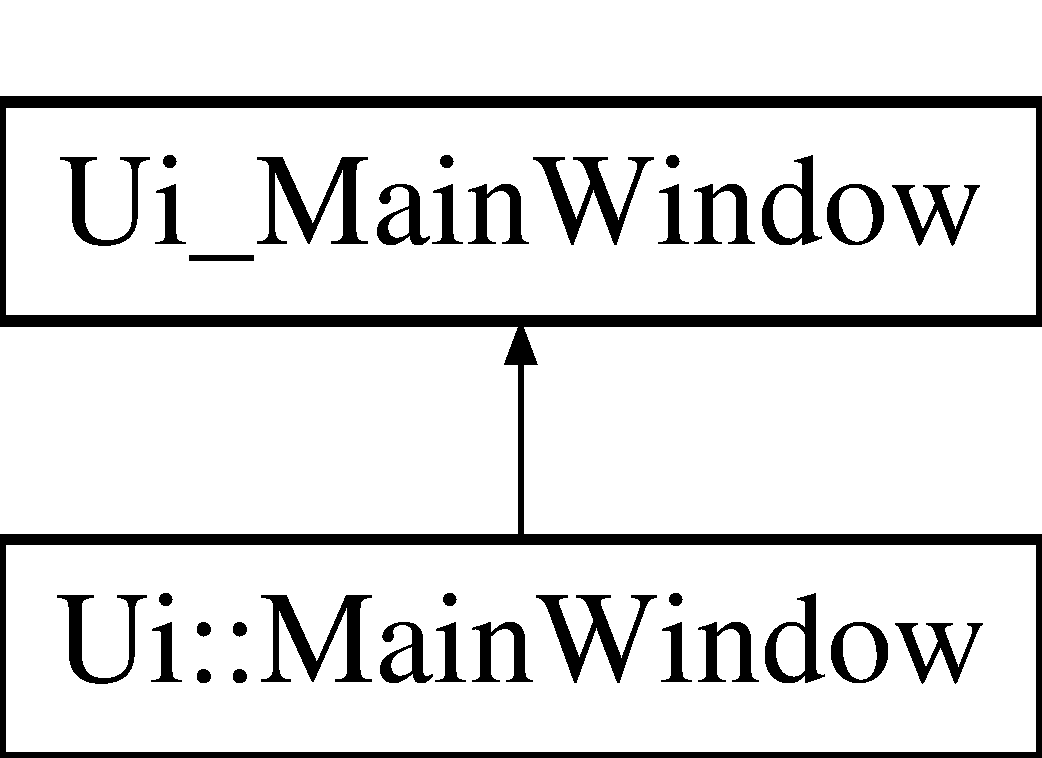
\includegraphics[height=2.000000cm]{class_ui___main_window}
\end{center}
\end{figure}
\subsection*{Public Member Functions}
\begin{DoxyCompactItemize}
\item 
\hypertarget{class_ui___main_window_acf4a0872c4c77d8f43a2ec66ed849b58}{void {\bfseries setup\-Ui} (Q\-Main\-Window $\ast$\hyperlink{class_main_window}{Main\-Window})}\label{class_ui___main_window_acf4a0872c4c77d8f43a2ec66ed849b58}

\item 
\hypertarget{class_ui___main_window_a097dd160c3534a204904cb374412c618}{void {\bfseries retranslate\-Ui} (Q\-Main\-Window $\ast$\hyperlink{class_main_window}{Main\-Window})}\label{class_ui___main_window_a097dd160c3534a204904cb374412c618}

\end{DoxyCompactItemize}
\subsection*{Public Attributes}
\begin{DoxyCompactItemize}
\item 
\hypertarget{class_ui___main_window_a30075506c2116c3ed4ff25e07ae75f81}{Q\-Widget $\ast$ {\bfseries central\-Widget}}\label{class_ui___main_window_a30075506c2116c3ed4ff25e07ae75f81}

\item 
\hypertarget{class_ui___main_window_a08a857edea57a9e53915f22187c06813}{Q\-Widget $\ast$ {\bfseries grid\-Layout\-Widget}}\label{class_ui___main_window_a08a857edea57a9e53915f22187c06813}

\item 
\hypertarget{class_ui___main_window_a525ed3c5fe0784ac502ee222fba4e205}{Q\-Grid\-Layout $\ast$ {\bfseries grid\-Layout}}\label{class_ui___main_window_a525ed3c5fe0784ac502ee222fba4e205}

\item 
\hypertarget{class_ui___main_window_a8eb0adb09460bff6ea84d805aa580db2}{Q\-Push\-Button $\ast$ {\bfseries btn\-Verificar}}\label{class_ui___main_window_a8eb0adb09460bff6ea84d805aa580db2}

\item 
\hypertarget{class_ui___main_window_ad9c89133780f28e6efa2ec17ceb9cff5}{Q\-Label $\ast$ {\bfseries label}}\label{class_ui___main_window_ad9c89133780f28e6efa2ec17ceb9cff5}

\item 
\hypertarget{class_ui___main_window_a7b9e75600981b2bfc14cc4485ee87371}{Q\-Line\-Edit $\ast$ {\bfseries txt\-\_\-nombre\-Jugador}}\label{class_ui___main_window_a7b9e75600981b2bfc14cc4485ee87371}

\item 
\hypertarget{class_ui___main_window_a2e2516d755e4dd53fc905dabddf2738a}{Q\-Label $\ast$ {\bfseries label\-\_\-2}}\label{class_ui___main_window_a2e2516d755e4dd53fc905dabddf2738a}

\item 
\hypertarget{class_ui___main_window_aeb911b62e28b6082ac2fd1d198e71e3e}{Q\-L\-C\-D\-Number $\ast$ {\bfseries lcd\-Tiempo}}\label{class_ui___main_window_aeb911b62e28b6082ac2fd1d198e71e3e}

\item 
\hypertarget{class_ui___main_window_a01be1e9ef33825ad8d509e2d545c2a01}{Q\-Label $\ast$ {\bfseries lbl\-M}}\label{class_ui___main_window_a01be1e9ef33825ad8d509e2d545c2a01}

\item 
\hypertarget{class_ui___main_window_a2be1c24ec9adfca18e1dcc951931457f}{Q\-Menu\-Bar $\ast$ {\bfseries menu\-Bar}}\label{class_ui___main_window_a2be1c24ec9adfca18e1dcc951931457f}

\item 
\hypertarget{class_ui___main_window_a5172877001c8c7b4e0f6de50421867d1}{Q\-Tool\-Bar $\ast$ {\bfseries main\-Tool\-Bar}}\label{class_ui___main_window_a5172877001c8c7b4e0f6de50421867d1}

\item 
\hypertarget{class_ui___main_window_a50fa481337604bcc8bf68de18ab16ecd}{Q\-Status\-Bar $\ast$ {\bfseries status\-Bar}}\label{class_ui___main_window_a50fa481337604bcc8bf68de18ab16ecd}

\end{DoxyCompactItemize}


The documentation for this class was generated from the following file\-:\begin{DoxyCompactItemize}
\item 
C\-:/\-Users/\-Janet/\-Documents/\-Git\-Hub/\-Final/build-\/\-Sudoku-\/\-Desktop\-\_\-\-Qt\-\_\-5\-\_\-0\-\_\-2\-\_\-\-Min\-G\-W\-\_\-32bit-\/\-Debug/ui\-\_\-mainwindow.\-h\end{DoxyCompactItemize}

%--- End generated contents ---

% Index
\newpage
\phantomsection
\addcontentsline{toc}{part}{Index}
\printindex

\end{document}
